\documentclass[article,30pt,extrafontsizes]{memoir}
\usepackage[none]{hyphenat}
\RequirePackage[utf8]{inputenc}
\RequirePackage[T1]{fontenc}
\RequirePackage{lmodern}
\RequirePackage{multicol}
\RequirePackage{graphicx}
\RequirePackage{lipsum}
\RequirePackage{blindtext}
\RequirePackage[svgnames,table]{xcolor}
\RequirePackage{tikz}
\RequirePackage[framemethod=tikz]{mdframed}
\RequirePackage{color}
\RequirePackage{geometry}
\RequirePackage{adjmulticol}
\RequirePackage[skins,most,listings,skins]{tcolorbox}

\RequirePackage{booktabs}
\RequirePackage{longtable}
\RequirePackage{array}
\RequirePackage{multirow}
\RequirePackage{wrapfig}
\RequirePackage{float}
\RequirePackage{colortbl}
\RequirePackage{pdflscape}
\RequirePackage{pagecolor}
\RequirePackage{tabu}
\RequirePackage{threeparttable}
\RequirePackage{threeparttablex}
\RequirePackage[normalem]{ulem}
\RequirePackage{makecell}
\RequirePackage{wrapfig}

%rof hyperrefs
\RequirePackage{hyperref}
\hypersetup{
    colorlinks=true,
    linkcolor=linkcol,
    citecolor=citecol,
    filecolor=linkcol,
    urlcolor=urlcol,
}
%For figure and table placement
\RequirePackage{float}
\floatplacement{figure}{H}
\floatplacement{table}{H}

%%%%%%%%% COLOURS %%%%%%%%
%Fill/ Line Colours
\definecolor{titleboxbgcol}{HTML}{7d0404}
\definecolor{titleboxbordercol}{HTML}{590303}
\definecolor{columnlinecol}{HTML}{fa7a7a}
\definecolor{bodybgcol}{HTML}{ffffff}
\definecolor{sectitlebgcol}{HTML}{7d0404}
\definecolor{sectitlebordercol}{HTML}{7d0404}
% Text Colours
\definecolor{titletextcol}{HTML}{ffffff}
\definecolor{authortextcol}{HTML}{fa7a7a}
\definecolor{affiliationtextcol}{HTML}{FFFFFF}
\definecolor{sectitletextcol}{HTML}{ffffff}
\definecolor{bodytextcol}{HTML}{000000}
\definecolor{footnotetextcol}{HTML}{ffffff}
\definecolor{citecol}{HTML}{CC0000}
\definecolor{urlcol}{HTML}{0e8bb5}
\definecolor{linkcol}{HTML}{FFFFFF}
\definecolor{tio}{HTML}{ffd1d7}

%Memoir spacing options
%spacing between figure/ table and caption
\setlength{\abovecaptionskip}{0.4in}
\setlength{\belowcaptionskip}{0.2in}
\captionnamefont{\footnotesize\sffamily\bfseries}
\captiontitlefont{\footnotesize\sffamily}

%define column options
\setlength{\columnseprule}{0.1pt}
\def\columnseprulecolor{\color{columnlinecol}}

%define section title features
\setsubsubsecheadstyle{\small\color{sectitletextcol}\textbf}% Set \section style
\setsecnumformat{}
\def\sectionmark#1{\markboth{#1}{#1}}

%%%%%%%%%%%% TCOLORBOXES TO THE RESCUE %%%%%%%%%%%%%%%%%%%%
%Title Box
\newtcolorbox{topbox}{
enhanced,
colback=titleboxbgcol,
colframe=titleboxbordercol,
halign=center,
boxrule=1cm,
sharp corners=all,
 overlay={
    \node[anchor=south west]
      at ([xshift=1in,yshift=1.5in]frame.south west)
       {
\includegraphics[width=3in]{imagenes/unsaac}};
    \node[anchor=south east]
      at ([xshift=-1in,yshift=1.5in]frame.south east)
       {
\includegraphics[width=3in]{imagenes/dui}};}

}
%Body Section Title Box
\newtcolorbox{myboxstuff}[1][]{
code={\parindent=0em},
colframe=sectitlebordercol,
nobeforeafter,
left skip=0pt,
valign=center,
halign=center,
fontupper=\Large\bfseries,
colupper=sectitletextcol,
boxrule=2mm,
colback=sectitlebgcol,
sharp corners=uphill, #1}
\newcommand{\mybox}[1]{%
\begin{myboxstuff}
\strut #1
\end{myboxstuff}%
}
\makeheadstyles{MyBox}{
    \setsecheadstyle{\mybox}
}
\headstyles{MyBox}\makepagestyle{MyBox}
%-----------------------------------------------------
%Make sure that the page is empty of any preset items from memoir
\thispagestyle{empty}

%biblatex options
\usepackage[style=authoryear,backend=bibtex]{biblatex}
\renewcommand*{\bibfont}{\small} %% SC
\bibliography{packages.bib}
\defbibheading{bibliography}[\bibname]{%
\setlength\bibitemsep{0.8\itemsep} %% SC
\section*{#1}%
\markboth{#1}{#1}}
\AtBeginDocument{%
  \renewcommand{\bibname}{Referencias}
}

%Remove section numbering & set 2nd level header as first level
%to avoid the automatic new page generated from memoir chapter
%formatting
\counterwithout{section}{chapter}
\makechapterstyle{mydefault}{
\addtocounter{secnumdepth}{2}
\setsecheadstyle{\mybox}
\setsubsecheadstyle{\itshape}
\setsubsubsecheadstyle{\itshape}
}

%set the chapterstyle
\chapterstyle{mydefault}

%define column spacing
\setlength\columnsep{0.5in}

%spacing params
\setlength\parindent{0em}
\setlength\parskip{0em}
\setlength\hangparas{0}

%spacing after section head title
\setaftersecskip{0em}
\setbeforesecskip{1.5em}
\setlength\textfloatsep{0in}
\setlength\floatsep{0in}
\setlength\intextsep{0in}

\setstocksize{47in}{33in}
\settrimmedsize{47in}{33in}{*}
\settypeblocksize{47in}{33in}{*}
\setlrmargins{*}{*}{1}
\setulmarginsandblock{2cm}{*}{*}
\setmarginnotes{0.5em}{1cm}{1cm}
\setlength{\footskip}{0cm}
\setlength{\footnotesep}{0cm}
\setlength{\headheight}{0pt}
\setlength{\headsep}{0pt}
\setlength{\trimtop}{0pt}
\setlength{\trimedge}{0pt}
\setlength{\uppermargin}{0pt}
\checkandfixthelayout
%Footnote to white
\RequirePackage{footmisc}
\def\footnotelayout{\centering\color{footnotetextcol}}

% see https://stackoverflow.com/a/47122900

% choose font family
\RequirePackage{mathptmx}

% define the BODYBGCOL
\newpagecolor{bodybgcol}

%sets footnote to be white hopefully
\renewcommand\footnoterule{}
\renewcommand{\thempfootnote}{\footnotesize\color{footnotetextcol}{\arabic{mpfootnote}}}

%-------------- Begin Document -------------------%
\begin{document}

%-------------- Title Box Start ------------------%
%tcolorbox allows for pictures hopefully
\begin{topbox}
  \color{titletextcol}
  \vspace{0.5in}
  \LARGE{\textsc{\textbf{Universidad Nacional de San Antonio Abad del Cusco}}
\break \textsc{\textbf{facultad de ciencias químicas, físicas y matemáticas}}
\break \textsc{dirección de la unidad de la unidad de investigación-fcqfm}
\break \textbf{Procesamiento de Lenguaje Natural (NLP) en el drama Ollantay}}  \\[0.3in]  %% SC
  \color{authortextcol} \Large{Chullo Oscar\textsuperscript{1} Zuñiga
Arturo\textsuperscript{2}} \\[0.2in] %% SC
  \color{affiliationtextcol} \large{\textsuperscript{1}E.P. de
Matemática, UNSAAC, Cusco, Perú; \textsuperscript{2}E.P. de Matemática,
UNSAAC, Cusco, Perú \break \textsuperscript{1}
\href{mailto:193029@unsaac.edu.pe}{\nolinkurl{193029@unsaac.edu.pe}};
\textsuperscript{2}
\href{mailto:arturo.zuniga@unsaac.edu.pe}{\nolinkurl{arturo.zuniga@unsaac.edu.pe}}} %% SC
  \vspace{1cm}
\end{topbox}
%--------------- Title Box End -------------------%
%----------------- Body Start --------------------%
% Begin body of poster
\sloppy 

\begin{multicols*}{3}
	
\large{  %% SC
\color{bodytextcol}
\section{Resumen}\label{resumen}

El propósito del siguiente póster es dar a conocer el \texttt{\colorbox{tio}{\textcolor{titleboxbgcol}{Procesamiento\ de\ Lenguaje\ Natural (NLP)}}} para el procesamiento de textos en el campo del \texttt{\colorbox{tio}{\textcolor{titleboxbgcol}{aprendizaje\ supervisado}}}, mostrándose una aplicación en el texto del drama Ollantay, en este se definen los \texttt{\colorbox{tio}{\textcolor{titleboxbgcol}{token}}} y \texttt{\colorbox{tio}{\textcolor{titleboxbgcol}{n-gramas}}} como unidades de análisis para conocer a rasgos generales un análisis preliminar del texto.

\vspace{0.5em}

\textbf{\emph{Palabras Clave:}} \emph{Procesamiento de Lenguaje Natural}, \emph{aprendizaje supervisado}, \emph{token}, \emph{n-gramas}.

\section{Introducción}\label{introducciuxf3n}

El \texttt{\colorbox{tio}{\textcolor{titleboxbgcol}{lenguaje natural}}} es un lenguaje desarrollado y evolucionado por los humanos a través del uso y comunicación ``natural''. Tal lenguaje puede ser expresado de manera escrita, verbal o incluso con signos.\autocite{salkar}

\vspace{0.5em}

El \texttt{\colorbox{tio}{\textcolor{titleboxbgcol}{procesamiento del lenguaje natural (NLP)}}} es un campo de estudio que se centra en la interacción entre el lenguaje natural y la computación, implica el uso de técnicas computacionales para analizar, comprender y generar texto o voz en lenguaje natural.

\section{Metodología}\label{metodologuxeda}

Para realizar los análisis en los textos (datos no estructurados, ver \textbf{Fig. 1}), se definen los \texttt{\colorbox{tio}{\textcolor{titleboxbgcol}{token}}} como unidad significativa de los textos, en términos de la minería de textos, un \texttt{\colorbox{tio}{\textcolor{titleboxbgcol}{token}}} puede almacenar una sola \texttt{\colorbox{tio}{\textcolor{titleboxbgcol}{palabra}}}, una conjugación de \texttt{\colorbox{tio}{\textcolor{titleboxbgcol}{n-gramas}}}, una \texttt{\colorbox{tio}{\textcolor{titleboxbgcol}{oración}}} o un \texttt{\colorbox{tio}{\textcolor{titleboxbgcol}{párrafo}}}.\autocite{silge}

\begin{center}
	\textbf{Figura 1:} \emph{Tipos de datos}
	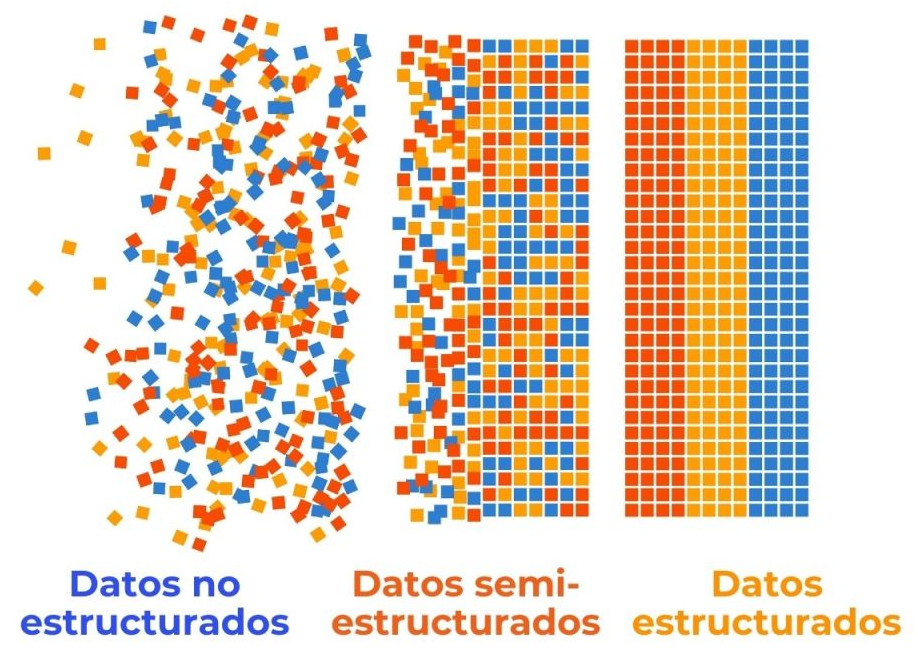
\includegraphics[width=9in]{imagenes/daaa.png}
\end{center}

Estructurar los datos de texto significa que se ajustan a los principios de datos ordenados y se pueden manipular con un conjunto de herramientas consistentes:
\begin{enumerate}
\def\labelenumi{\arabic{enumi}.}
\item
  \textbf{Cadena:} Como vectores de caracteres.
\item
  \textbf{Corpus:} Conjunto de cadenas sin procesar.
\item
  \textbf{Matriz de documentos y términos:} Describe un corpus con una fila para cada documento y una columna para cada término.
\end{enumerate}

Si queremos analizar un texto, se puede realizar el análisis de \texttt{\colorbox{tio}{\textcolor{titleboxbgcol}{token}}} por palabras individuales o por grupos de palabras, tomando en consideración el \texttt{\colorbox{tio}{\textcolor{titleboxbgcol}{token}}}, se puede evaluar un texto de forma sentimental (ver \textbf{Fig. 2}), para así clasificar si el \texttt{\colorbox{tio}{\textcolor{titleboxbgcol}{token}}} es \texttt{\colorbox{tio}{\textcolor{titleboxbgcol}{positivo}}} o \texttt{\colorbox{tio}{\textcolor{titleboxbgcol}{negativo}}}, o considerar otros criterios de evaluación.

\begin{center}
	\textbf{Figura 2:} \emph{Diagrama de flujo de un análisis de texto para el análisis de sentimientos}
	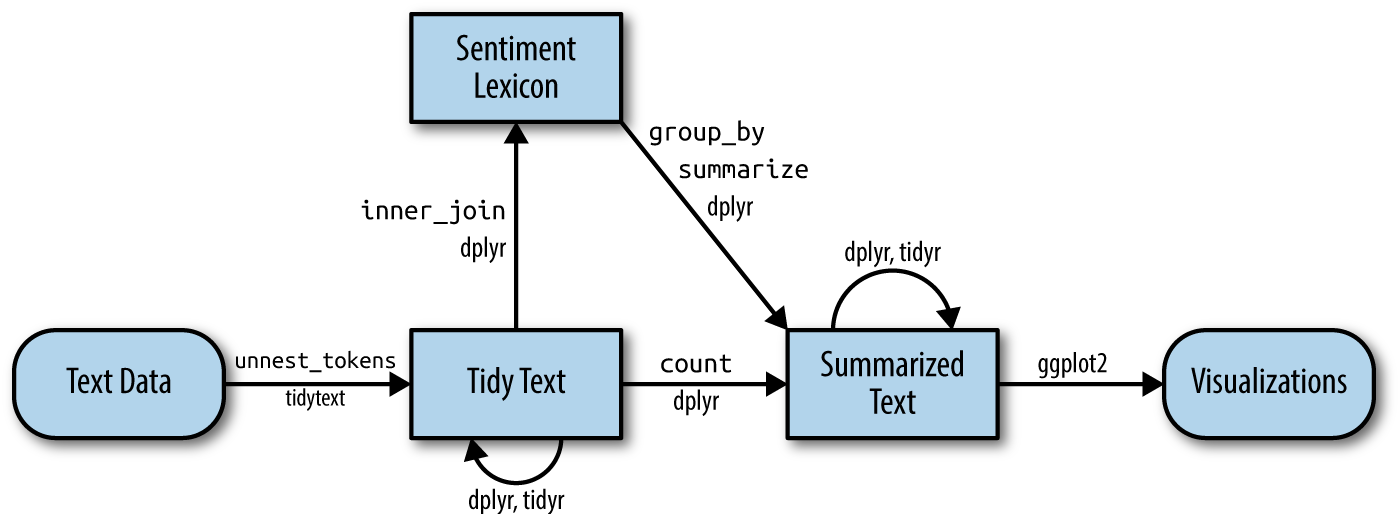
\includegraphics[width=8in]{imagenes/sent.png}
\end{center}

En caso se quiera hacer un análisis para evaluar los \texttt{\colorbox{tio}{\textcolor{titleboxbgcol}{token}}} y su relación entre si, se recurre a los \texttt{\colorbox{tio}{\textcolor{titleboxbgcol}{n-gramas}}} para examinar que \texttt{\colorbox{tio}{\textcolor{titleboxbgcol}{token}}} tienden a seguir a otros, dependiendo del número de \texttt{\colorbox{tio}{\textcolor{titleboxbgcol}{token}}} se emplean los sufijos:  \texttt{\colorbox{tio}{\textcolor{titleboxbgcol}{Bi}}}, \texttt{\colorbox{tio}{\textcolor{titleboxbgcol}{Tri}}}, \texttt{\colorbox{tio}{\textcolor{titleboxbgcol}{Tetra}}}, etc.

\vspace{0.5em}

\textbf{Bi-grama}

$$X\longrightarrow Y$$

\vspace{0.5em}

\textbf{Tri-grama}

$$X\longrightarrow Y\longrightarrow Z$$

Para realizar un análisis de textos, en el software R se puede acceder a la colección \texttt{\colorbox{tio}{\textcolor{titleboxbgcol}{Proyecto Gutenberg}}} mediante el paquete \texttt{\colorbox{tio}{\textcolor{titleboxbgcol}{gutenbergr}}}, del cual se ha extraído la versión traducida al Inglés del drama \texttt{\colorbox{tio}{\textcolor{titleboxbgcol}{Ollantay}}}. El cual se consideró como la base de datos textuales a analizar mediante el \texttt{\colorbox{tio}{\textcolor{titleboxbgcol}{NLP}}}.

\section{Resultados}\label{resultados}

\textbf{Análisis de sentimientos}

El drama \texttt{\colorbox{tio}{\textcolor{titleboxbgcol}{Ollantay}}} nos presenta una narrativa sobre el amor, la justicia y la lucha social. Con un análisis de \texttt{\colorbox{tio}{\textcolor{titleboxbgcol}{token}}}, se obtuvieron los resultados que se muestran en \textbf{Fig. 3} y \textbf{Fig. 4}.

\begin{center}
	\textbf{Figura 3:} \emph{Clasificación de sentimientos}
		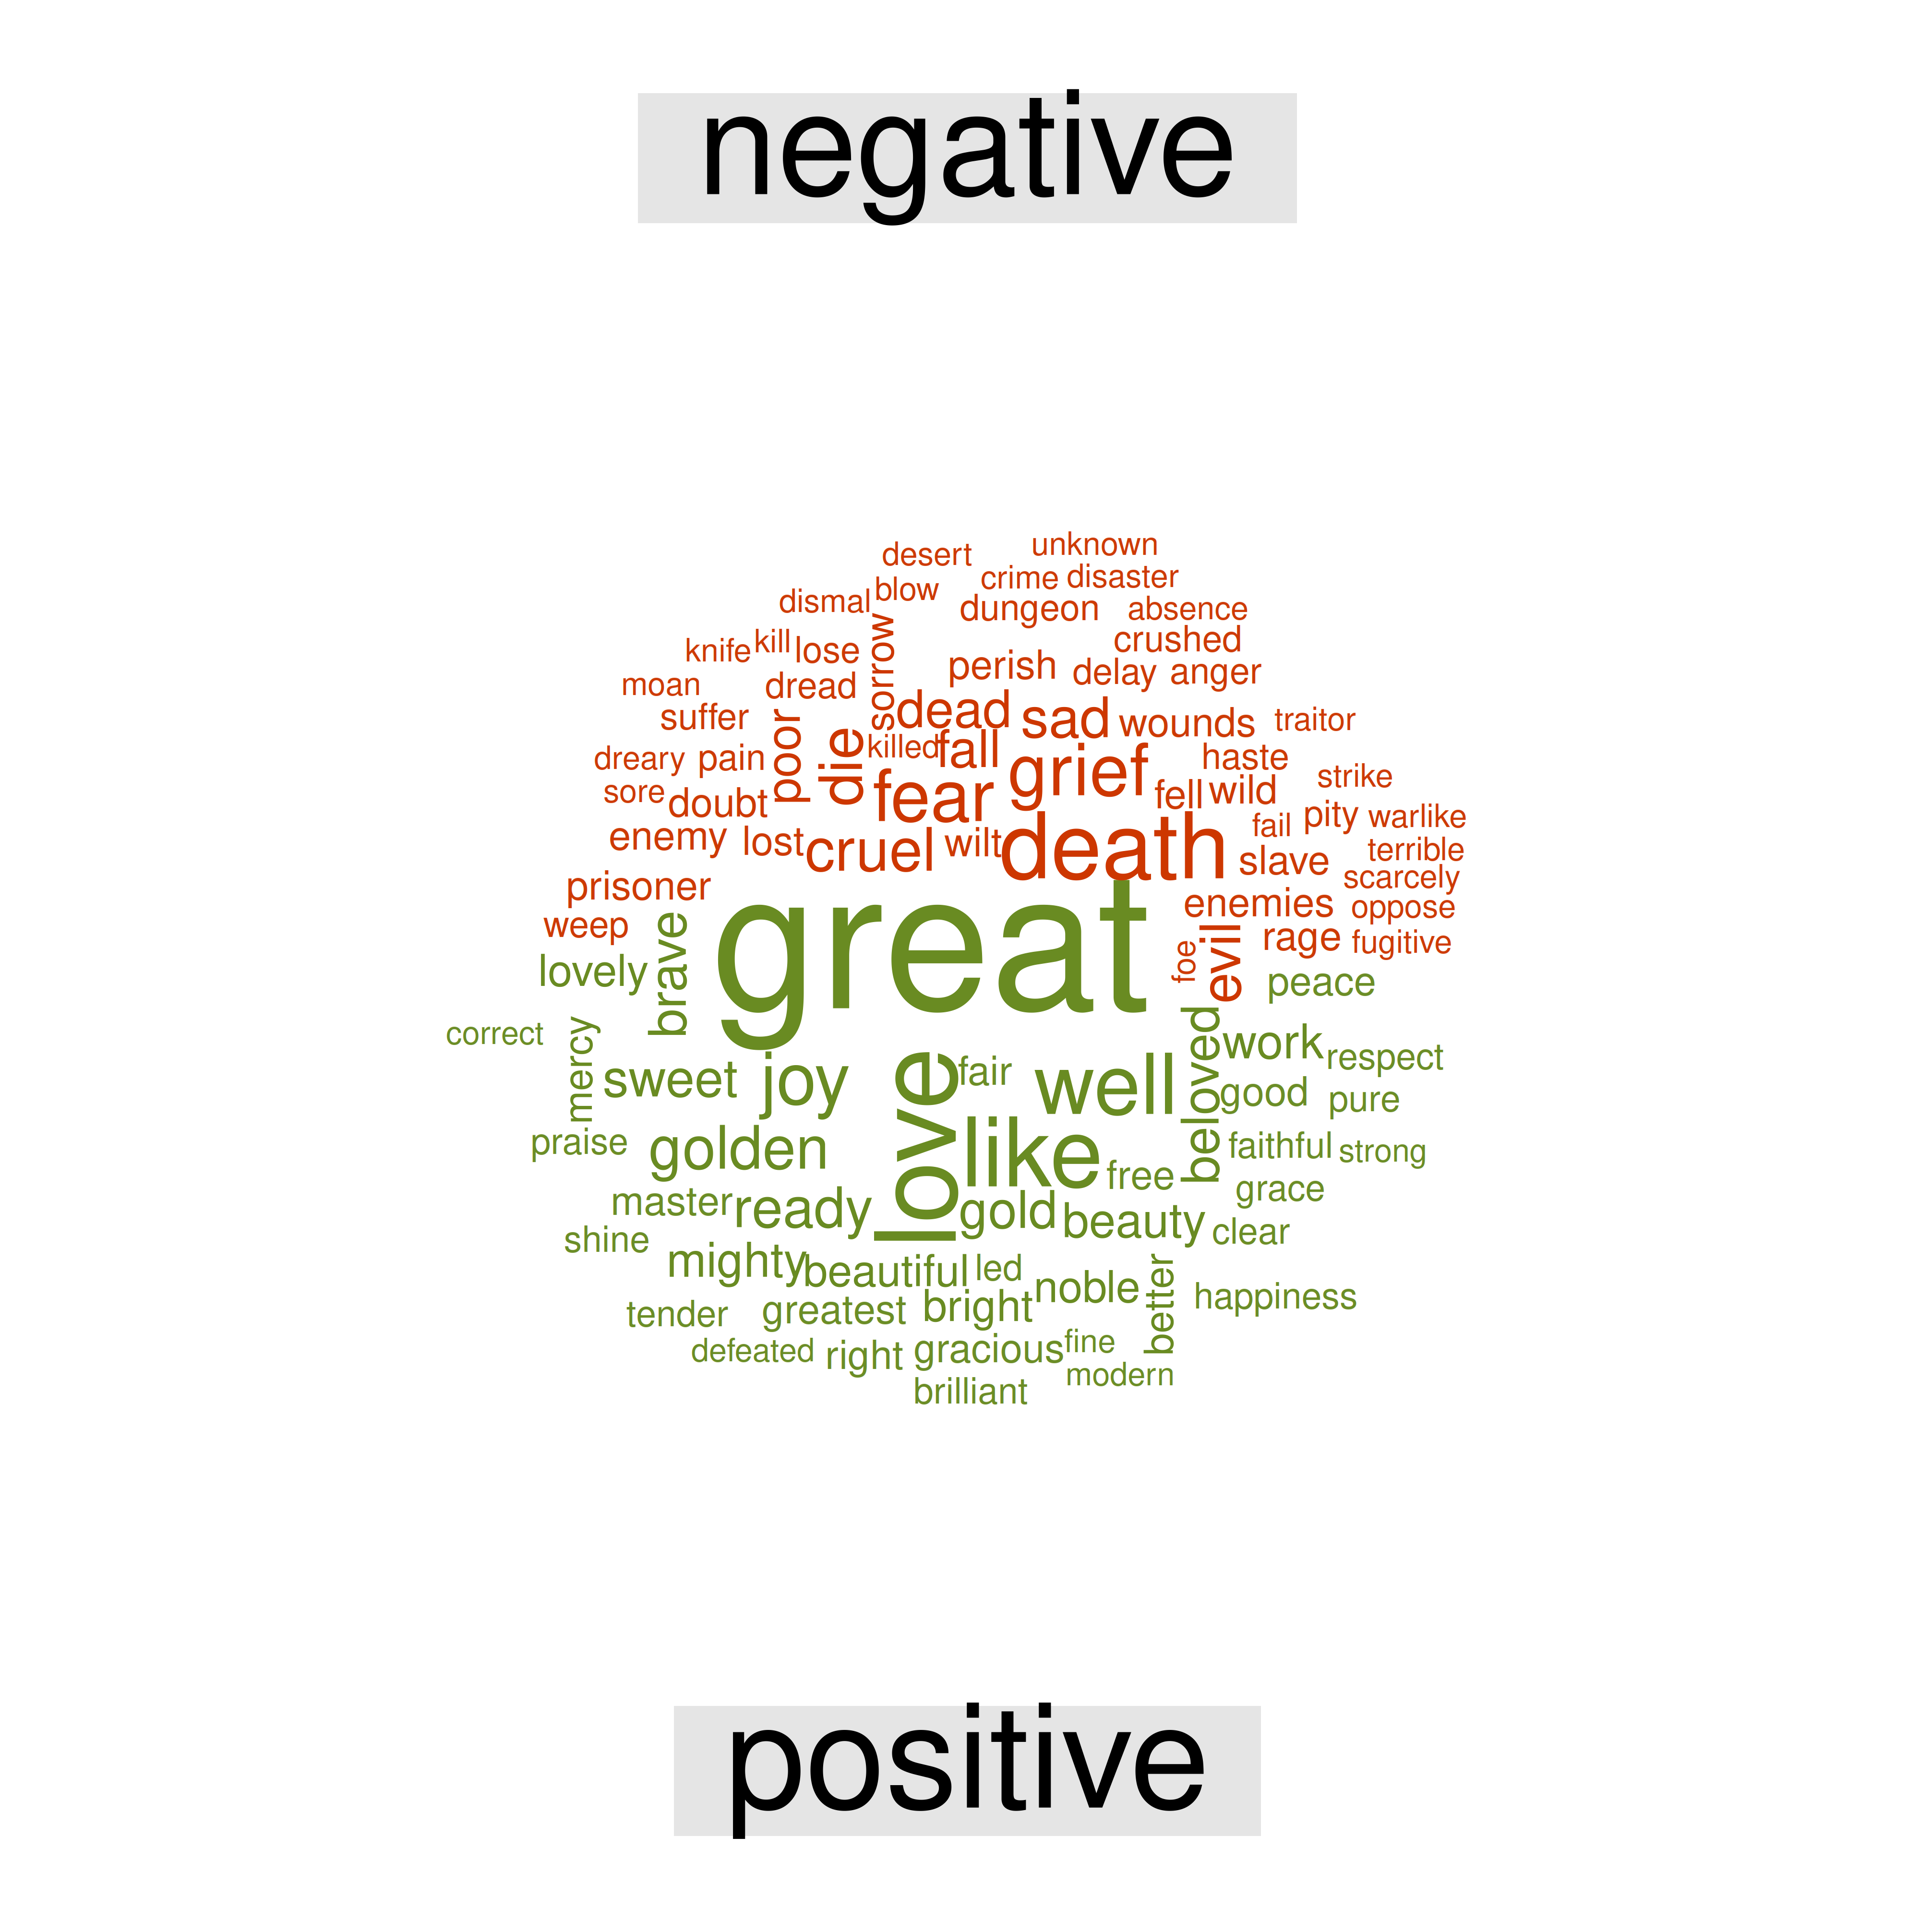
\includegraphics[width=9in]{senti_001.png}
\end{center}

\begin{center}
	\textbf{Figura 4:} \emph{Valoración de sentimientos con bi-gramas}
		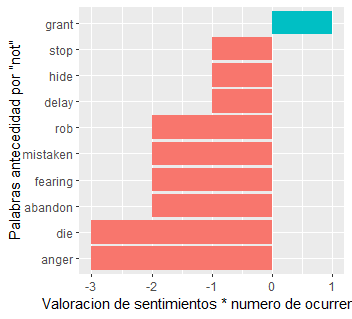
\includegraphics[width=8in]{Rplot.png}
\end{center}

\textbf{Análisis de n-gramas}
Se han establecido los \texttt{\colorbox{tio}{\textcolor{titleboxbgcol}{token}}} con todas las palabras de la obra, al cual se hizo un analisis por \texttt{\colorbox{tio}{\textcolor{titleboxbgcol}{Bi-gramas}}} (ver \textbf{Fig. 5}) y \texttt{\colorbox{tio}{\textcolor{titleboxbgcol}{Tri-gramas}}} (ver \textbf{Fig. 6})

\begin{center}
	\textbf{Figura 5:} \emph{Análisis correlacional de palabras con bi-gramas}
	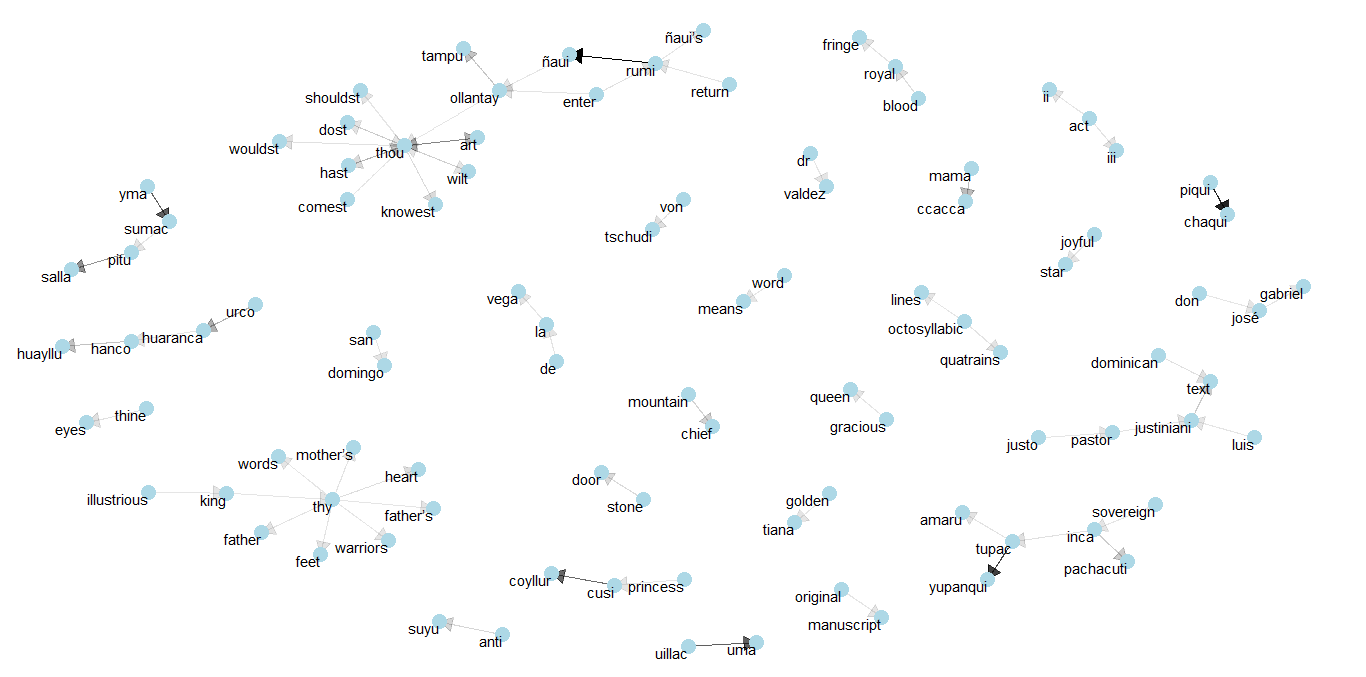
\includegraphics[width=9in]{piquas.png}
\end{center}

\begin{center}
	\textbf{Figura 6:} \emph{Análisis correlacional de palabras con tri-gramas}
	
	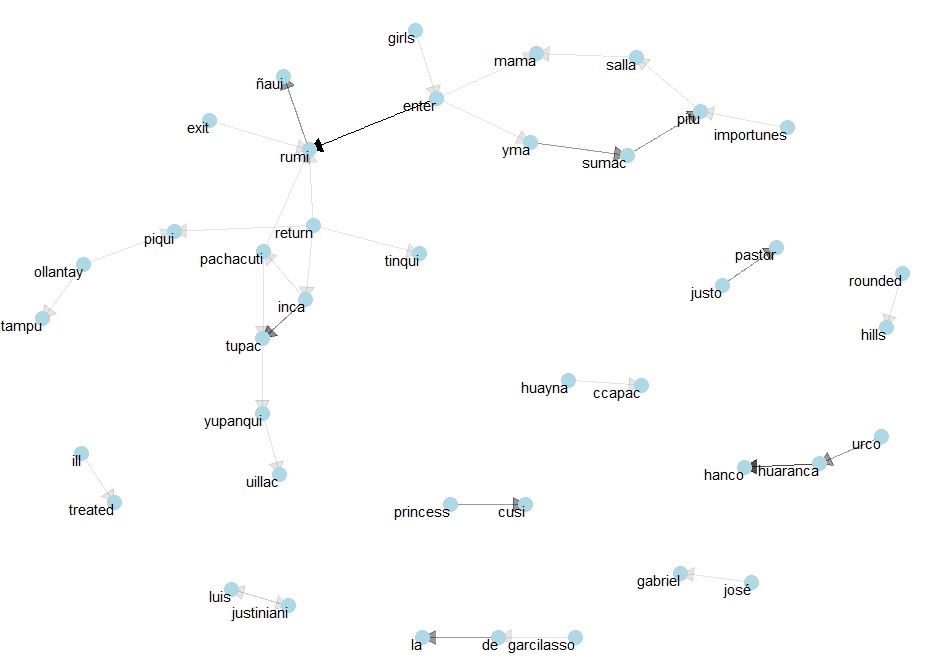
\includegraphics[width=8in]{de.jpeg}
\end{center}

\section{Conclusión}\label{conclusiuxf3n}

\begin{enumerate}
\def\labelenumi{\arabic{enumi}.}
\item
  Con el análisis de sentimientos, se pudieron identificar sentimientos \texttt{\colorbox{tio}{\textcolor{titleboxbgcol}{positivos}}} y \texttt{\colorbox{tio}{\textcolor{titleboxbgcol}{negativos}}} el cual guardan relación con la idea general de la obra. Sin embargo, cabe resaltar que un análisis con \texttt{bi-gramas} es efectivo para identificar adecuadamente los sentimientos.
\item
  En el análisis de los \texttt{n-gramas} se ha podido ver que un
  análisis con \texttt{bi-gramas} es más explicativo que por \texttt{tri-gramas}.
\end{enumerate}
}

\printbibliography
\end{multicols*}
%------------------ Body End ---------------------%
%end the poster
\end{document}
